% Generated semantic source for AI Almanach v3.
% Edit v3 directly after initial generation; do not overwrite
% editorial changes by rerunning the converter casually.

% ==== Visualization =============================================================================
\chapter{Visualization}

\chapterlead{How can a visual make evidence clearer without overstating it?}{Question}{Encode}{Compare}{Explain}{visualization}

% ==== Section 1: Foundations of Data Visualization ==========================================
\section{Foundations of Data Visualization}

% ---- 19.1.1 Why Visualization Matters ------------------------------------------------------
\subsection{Why Visualization Matters}

\begin{v3topic}{Anscombe's Quartet}
    Anscombe's Quartet (1973) is four datasets that share nearly identical summary statistics
    ($\bar{x}=9$, $\bar{y}\approx7.5$, $r\approx0.816$, same regression line) yet look
    entirely different when plotted. It is the canonical argument for always visualizing data
    before modelling\textsuperscript{\cite[][pp.~4--6]{downeyThinkStatsExploratory2015}}.
\visualseparator
    \begin{center}
    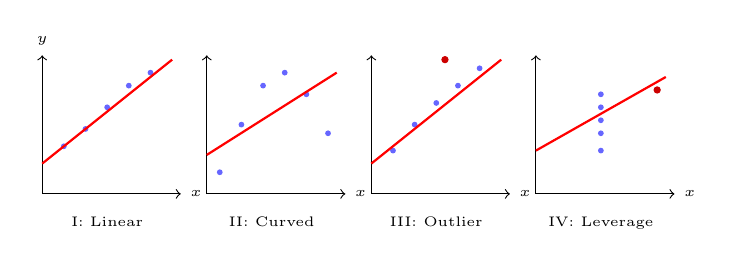
\begin{tikzpicture}[scale=0.55]
        % Dataset I
        \begin{scope}[xshift=0cm]
            \draw[->] (0,0)--(3.2,0) node[right,font=\tiny]{$x$};
            \draw[->] (0,0)--(0,3.2) node[above,font=\tiny]{$y$};
            \foreach \x/\y in {0.5/1.1,1.0/1.5,1.5/2.0,2.0/2.5,2.5/2.8}
                \filldraw[blue!60] (\x,\y) circle (1.5pt);
            \draw[red,thick] (0,0.7)--(3,3.1);
            \node[font=\tiny,below] at (1.5,-0.3) {I: Linear};
        \end{scope}
        % Dataset II
        \begin{scope}[xshift=3.8cm]
            \draw[->] (0,0)--(3.2,0) node[right,font=\tiny]{$x$};
            \draw[->] (0,0)--(0,3.2);
            \foreach \x/\y in {0.3/0.5,0.8/1.6,1.3/2.5,1.8/2.8,2.3/2.3,2.8/1.4}
                \filldraw[blue!60] (\x,\y) circle (1.5pt);
            \draw[red,thick] (0,0.9)--(3,2.8);
            \node[font=\tiny,below] at (1.5,-0.3) {II: Curved};
        \end{scope}
        % Dataset III
        \begin{scope}[xshift=7.6cm]
            \draw[->] (0,0)--(3.2,0) node[right,font=\tiny]{$x$};
            \draw[->] (0,0)--(0,3.2);
            \foreach \x/\y in {0.5/1.0,1.0/1.6,1.5/2.1,2.0/2.5,2.5/2.9}
                \filldraw[blue!60] (\x,\y) circle (1.5pt);
            \filldraw[red!80!black] (1.7,3.1) circle (2pt);
            \draw[red,thick] (0,0.7)--(3,3.1);
            \node[font=\tiny,below] at (1.5,-0.3) {III: Outlier};
        \end{scope}
        % Dataset IV
        \begin{scope}[xshift=11.4cm]
            \draw[->] (0,0)--(3.2,0) node[right,font=\tiny]{$x$};
            \draw[->] (0,0)--(0,3.2);
            \foreach \y in {1.0,1.4,1.7,2.0,2.3}
                \filldraw[blue!60] (1.5,\y) circle (1.5pt);
            \filldraw[red!80!black] (2.8,2.4) circle (2pt);
            \draw[red,thick] (0,1.0)--(3,2.7);
            \node[font=\tiny,below] at (1.5,-0.3) {IV: Leverage};
        \end{scope}
    \end{tikzpicture}
\captionof{figure}{Why Visualization Matters: Anscombe's Quartet.}
\label{fig:ch18-visualization-inline-01}
    \end{center}

\end{v3topic}
\begin{v3topic}{Pre-attentive Processing and Cognitive Load}
    Human vision processes certain visual features in parallel, \emph{before} conscious
    attention --- these are called \textbf{pre-attentive attributes}: colour hue, luminance,
    size, orientation, motion, and spatial position. A visualization that exploits
    pre-attentive attributes communicates faster because the viewer does not need to
    ``read'' each element.
    \textbf{Cognitive load} is the mental effort required to interpret a chart.
    Good design minimizes extraneous load (decorative elements, 3-D perspectives, grid
    clutter) so working memory is free for the task of understanding the
    data\textsuperscript{\cite[][pp.~25--40]{jansenHandbuchInfografik1999}}.

\end{v3topic}
\begin{v3topic}{Data-Ink Ratio (Tufte)}
    Edward Tufte defined the \textbf{data-ink ratio} as the proportion of a graphic's ink
    devoted to displaying data:
    \begin{equation}
        \text{data-ink ratio} = \frac{\text{ink used to display data}}{\text{total ink in graphic}}
    \end{equation}
    \textbf{Maximize} this ratio by erasing non-data ink (chart borders, redundant tick marks,
    background fills) and by erasing redundant data-ink (repeat labels, heavy gridlines).
    The complementary concept is \textbf{chartjunk}: visual elements that convey no
    information yet consume ink and attention.

\end{v3topic}
\begin{v3topic}{Exploratory vs.\ Explanatory Visualization}
    \begin{tblr}{|X[l]|X[l]|}
        \hline
        \textbf{Exploratory}                   & \textbf{Explanatory}                    \\
        \hline
        Analyst audience                       & Stakeholder / public audience           \\
        \hline
        Quick, rough, many charts              & Polished, focused, few charts           \\
        \hline
        Find the signal in the data            & Communicate a specific insight          \\
        \hline
        Default library themes acceptable      & Deliberate design choices required      \\
        \hline
        Tools: notebooks, pandas, seaborn      & Tools: Plotly, Flourish, Tableau        \\
        \hline
    \end{tblr}
\captionof{table}{Why Visualization Matters: Exploratory vs.\ Explanatory Visualization.}
\label{tab:ch18-visualization-inline-01}
    Most ML work is exploratory; results presentations require explanatory
    quality\textsuperscript{\cite[][pp.~1--18]{loducaDataStorytellingAltair2024}}.
\end{v3topic}

% ---- 19.1.2 Visual Encoding ----------------------------------------------------------------
\subsection{Visual Encoding}

\begin{v3topic}{Marks and Channels}
    A visualization encodes data values using \textbf{marks} (geometric primitives) and
    \textbf{channels} (visual properties of those marks).
    Common marks: \emph{points}, \emph{lines}, \emph{areas}, \emph{bars}, \emph{glyphs}.
    Common channels: \emph{position (x, y)}, \emph{length}, \emph{angle}, \emph{area},
    \emph{colour hue}, \emph{colour luminance}, \emph{saturation}, \emph{texture},
    \emph{shape}.
    The effectiveness of a channel depends on the type of data (quantitative, ordinal,
    nominal) and the perceptual task it must
    support\textsuperscript{\cite[][pp.~30--50]{jansenHandbuchInfografik1999}}.

\end{v3topic}
\begin{v3topic}{Cleveland \& McGill Effectiveness Ranking}
    Cleveland and McGill (1984) ranked channels by accuracy of magnitude estimation from
    most accurate to least:
    \begin{enumerate}
        \item Position along a common scale (bar chart, scatter)
        \item Position on identical but non-aligned scales
        \item Length
        \item Angle / slope
        \item Area
        \item Volume / curvature
        \item Colour shading / density
    \end{enumerate}
    \textbf{Implication}: prefer bar charts over pie charts (length vs.\ angle); prefer
    scatter plots over bubble charts when comparing magnitudes.

\end{v3topic}
\begin{v3topic}{Gestalt Principles in Chart Design}
    The Gestalt principles describe how humans group visual elements
    automatically:
    \par\smallskip\noindent
    \begin{tblr}{width=\linewidth,colspec={X[l,1]X[l,3]X[l,2]},
                 hlines,vlines}
        \hline
        \textbf{Principle}  & \textbf{Description}                                      & \textbf{Chart application}                      \\
        \hline
        Proximity           & Elements close together are perceived as a group          & Group bars in a clustered bar chart             \\
        \hline
        Similarity          & Elements with shared colour/shape are grouped             & Colour encodes category consistently            \\
        \hline
        Closure             & Open shapes are completed by the brain                    & Outline a region without filling it             \\
        \hline
        Continuity          & Elements on a smooth path are perceived as connected      & Line charts imply temporal sequence             \\
        \hline
        Figure/Ground       & Objects stand out from their background                   & Light background with dark marks                \\
        \hline
        Common Fate         & Objects moving together are grouped                       & Animated transitions in interactive vis         \\
        \hline
    \end{tblr}
\captionof{table}{Visual Encoding: Gestalt Principles in Chart Design.}
\label{tab:ch18-visualization-inline-02}
\end{v3topic}

% ---- 19.1.3 Colour in Visualization --------------------------------------------------------
\subsection{Colour in Visualization}

\begin{v3topic}{Colour Palette Types}
    Three palette families serve different data types:
    \begin{itemize}
        \item \textbf{Sequential} (e.g.\ Blues, viridis): for ordered data ranging from low to
              high. Luminance increases monotonically.
        \item \textbf{Diverging} (e.g.\ RdBu, coolwarm): for data with a meaningful midpoint
              (zero, mean). Hue diverges from a neutral centre.
        \item \textbf{Categorical / Qualitative} (e.g.\ tab10, Set2): for nominal groups.
              Uses distinct hues at similar luminance so no category appears more important.
    \end{itemize}
    Never apply a sequential palette to categorical data --- it implies an ordering that
    does not exist\textsuperscript{\cite[][pp.~120--135]{jansenHandbuchInfografik1999}}.

\end{v3topic}
\begin{v3topic}{Perceptual Uniformity and Colourblind Safety}
    A \textbf{perceptually uniform} palette maps equal numeric differences to equal
    perceptual differences in colour space (CIELAB). The \textbf{viridis} family
    (viridis, plasma, inferno, magma) was designed for perceptual uniformity and
    colourblind safety. Approximately 8\,\% of males are red-green colourblind (deuteranopia /
    protanopia). Safe practices:
    \begin{itemize}
        \item Avoid red-green pairings as the sole encoding
        \item Add a secondary channel (shape, line style) for critical distinctions
        \item Use \textbf{ColorBrewer} palettes which mark colourblind-safe options
        \item Test with a simulator (e.g.\ Coblis, colorblindr R package)
    \end{itemize}
\end{v3topic}

% ==== Section 2: Chart Types and When to Use Them ===========================================
\section{Chart Types and When to Use Them}

% ---- 19.2.1 Comparison and Distribution ---------------------------------------------------
\subsection{Comparison and Distribution}

\begin{v3topic}{Bar and Column Charts}
    \textbf{Bar charts} encode a quantitative value per category using bar length ---
    the most accurately decoded channel after position. Rules:
    \begin{itemize}
        \item Always start the y-axis at zero (truncating creates misleading area)
        \item Sort bars by value unless category order is meaningful
        \item Use horizontal bars when category labels are long
        \item \textbf{Grouped} bars: compare across sub-groups side by side
        \item \textbf{Stacked} bars: show part-to-whole; use sparingly, only when
              the total matters
    \end{itemize}
    Avoid 3-D bars, exploding slices, and gradient fills --- they add no
    information\textsuperscript{\cite[][pp.~60--75]{brucePracticalStatisticsData2017}}.

\end{v3topic}
\begin{v3topic}{Histograms and Density Plots}
    A \textbf{histogram} bins continuous data and plots frequency (or density) per bin.
    Bin width selection is critical: too wide hides shape, too narrow is noisy.
    Common rules:
    \begin{itemize}
        \item \textbf{Sturges}: $k = \lceil \log_2 n \rceil + 1$
        \item \textbf{Scott}: $h = 3.49\,\hat{\sigma}\,n^{-1/3}$
        \item \textbf{Freedman-Diaconis}: $h = 2\,\text{IQR}\,n^{-1/3}$
    \end{itemize}
    A \textbf{KDE (kernel density estimate)} smooths the histogram into a continuous
    density curve using a bandwidth $h$. Use KDE to compare distributions across
    groups where histogram bins would
    misalign\textsuperscript{\cite[][pp.~45--50]{downeyThinkStatsExploratory2015}}.

\end{v3topic}
\begin{v3topic}{Box Plots and Violin Plots}
    A \textbf{box plot} (Tukey, 1977) summarises a distribution with five statistics:
    minimum, Q1, median, Q3, maximum. Whiskers typically extend to
    $1.5\times\text{IQR}$; outliers are plotted individually.
    A \textbf{violin plot} adds a mirrored KDE to each side, revealing the full shape
    including multimodality --- information a box plot discards.
    A \textbf{strip / swarm plot} overlays actual data points on a box or violin.
    \textbf{Rule}: for $n < 50$, show raw points; for $50 < n < 1000$, violin +
    box; for $n > 1000$, box alone is
    sufficient\textsuperscript{\cite[][pp.~52--55]{downeyThinkStatsExploratory2015}}.

\end{v3topic}
\begin{v3topic}{When to Use Which Distribution Chart}
    \factvisual{
        \textbf{Start from the analytical question.}
        \begin{itemize}
            \item Need the shape of one continuous variable? Use a histogram or density.
            \item Need robust group comparison? Use box or violin plots.
            \item Need every observation? Use dots, strips, or swarms.
            \item Need category counts? Use bars, not a histogram.
        \end{itemize}
    }{
        \begin{tikzpicture}[node distance=4mm]
            \node[almanach accent card,text width=28mm] (q)
                {What must the reader compare?};
            \node[almanach card,text width=20mm,below left=7mm and 8mm of q]
                (shape) {shape};
            \node[almanach card,text width=20mm,below=7mm of q]
                (groups) {groups};
            \node[almanach card,text width=20mm,below right=7mm and 8mm of q]
                (points) {points};
            \node[almanach card,text width=20mm,below=of shape]
                (hist) {histogram / KDE};
            \node[almanach card,text width=20mm,below=of groups]
                (box) {box / violin};
            \node[almanach card,text width=20mm,below=of points]
                (strip) {strip / swarm};
            \draw[almanach arrow] (q) -- (shape);
            \draw[almanach arrow] (q) -- (groups);
            \draw[almanach arrow] (q) -- (points);
            \draw[almanach arrow] (shape) -- (hist);
            \draw[almanach arrow] (groups) -- (box);
            \draw[almanach arrow] (points) -- (strip);
        \end{tikzpicture}
        \visualcaption{Chart selection begins with the comparison task, then
          chooses the simplest mark that exposes the required evidence.}
          {fig:distribution-chart-decision-tree}
    }
    \begin{tblr}{|X[l]|X[l]|}
        \hline
        \textbf{Goal}                        & \textbf{Chart type}                    \\
        \hline
        Show overall shape                   & Histogram / KDE                        \\
        \hline
        Compare distributions across groups  & Violin or box plot                     \\
        \hline
        Identify outliers precisely          & Box plot with jitter                   \\
        \hline
        Show all data points ($n<200$)       & Strip / swarm plot                     \\
        \hline
        Compare frequencies across categories & Bar chart                             \\
        \hline
        Show ranking                         & Sorted horizontal bar chart            \\
        \hline
    \end{tblr}
\captionof{table}{Comparison and Distribution: When to Use Which Distribution Chart.}
\label{tab:ch18-visualization-inline-03}
\end{v3topic}

% ---- 19.2.2 Relationships and Correlation -------------------------------------------------
\subsection{Relationships and Correlation}

\begin{v3topic}{Scatter Plots and Bubble Charts}
    A \textbf{scatter plot} maps two quantitative variables to x and y position ---
    the most effective encoding for both. Use it to:
    \begin{itemize}
        \item Detect linear or non-linear relationships
        \item Identify clusters, gaps, and outliers
        \item Overlay a regression line or confidence band
    \end{itemize}
    A \textbf{bubble chart} adds a third variable via point area. Limitations:
    area is a weak channel (step 5 in Cleveland-McGill); prefer colour or
    a faceted scatter instead when precision matters.
    For large $n$ with overplotting: use 2-D binning (hexbin) or contour
    layers\textsuperscript{\cite[][pp.~80--90]{brucePracticalStatisticsData2017}}.

\end{v3topic}
\begin{v3topic}{Heatmaps and Correlation Matrices}
    A \textbf{heatmap} encodes a matrix of values using colour. Applications:
    \begin{itemize}
        \item \textbf{Correlation matrix}: $r_{ij} \in [-1, 1]$ for each feature pair;
              use a diverging palette centred at zero
        \item \textbf{Confusion matrix} (see Section~2.4): colour encodes prediction counts
        \item \textbf{Time $\times$ category}: e.g.\ weekly crime rates by weekday and hour
    \end{itemize}
    Cluster rows and columns with hierarchical clustering to reveal block structure.
    Annotate cells with numeric values when precision is needed.
    Never use a rainbow palette for heatmaps --- it introduces artificial
    boundaries\textsuperscript{\cite[][pp.~148--160]{molinHandsonDataAnalysis2021}}.

\end{v3topic}
\begin{v3topic}{Pair Plots (Scatterplot Matrix)}
    A \textbf{pair plot} (SPLOM) shows scatter plots for every pair of numeric features in a
    grid. Diagonal cells typically show the univariate distribution (histogram or KDE).
    Use pair plots early in EDA to:
    \begin{itemize}
        \item Survey all pairwise relationships at once
        \item Colour by class label to see linear separability
        \item Detect collinearity before regression or PCA
    \end{itemize}
    \textbf{Seaborn} provides \texttt{sns.pairplot(df, hue=``class'')} as a one-liner.
    For high-dimensional data ($p > 15$) pair plots become unwieldy --- switch to
    correlation heatmaps or dimensionality
    reduction\textsuperscript{\cite[][pp.~161--165]{molinHandsonDataAnalysis2021}}.
\end{v3topic}

% ---- 19.2.3 Composition and Time Series ---------------------------------------------------
\subsection{Composition and Time Series}

\begin{v3topic}{Pie Charts and When to Avoid Them}
    Pie charts encode part-to-whole proportions as angles. Humans are poor at comparing
    non-adjacent angles and estimating proportions less than 5\,\% or more than 70\,\%.
    \textbf{Prefer a stacked bar} when:
    \begin{itemize}
        \item More than 4--5 slices are needed
        \item Two pies must be compared
        \item Small differences between slices matter
    \end{itemize}
    A pie chart is acceptable only when: there are $\leq3$ slices, exact values are
    labeled, and the message is simply ``A is more than half''.
    A \textbf{donut chart} adds no information over a pie and the central hole
    can mislead about total
    area\textsuperscript{\cite[][pp.~95--100]{brucePracticalStatisticsData2017}}.

\end{v3topic}
\begin{v3topic}{Line Charts and Time Series}
    Line charts connect ordered observations and are the canonical choice for
    \textbf{time series}. Design guidelines:
    \begin{itemize}
        \item Start y-axis at zero only when the baseline is meaningful (counts, prices);
              for rates or ratios, show the range of variation
        \item Use \textbf{direct labels} on lines instead of a legend when $\leq5$ series
        \item Add \textbf{reference lines} or shaded bands to mark events (model release,
              policy change, lockdown)
        \item \textbf{Sparklines}: miniaturised line charts embedded in text or tables to
              show trend without axes
        \item For seasonal data: plot seasonal decomposition (trend + seasonal + residual)
              rather than the raw series
    \end{itemize}
\end{v3topic}

% ---- 19.2.4 Specialized ML Visualizations -------------------------------------------------
\subsection{Specialized ML Visualizations}

\begin{v3topic}{Confusion Matrix}
    A confusion matrix is a $K \times K$ table of true vs.\ predicted class labels.
    For binary classification:
    \begin{equation}
        \begin{pmatrix} \text{TN} & \text{FP} \\ \text{FN} & \text{TP} \end{pmatrix}
    \end{equation}
    Visualize as a heatmap with count and row-normalized percentage annotations.
    Normalization reveals class-level error rates independently of class imbalance.
    Common errors visible: systematic confusion between two classes (off-diagonal hot
    spots); high false-negative rate (dangerous in medical
    screening)\textsuperscript{\cite[][pp.~180--185]{raschkaPythonMachineLearning2015}}.

\end{v3topic}
\begin{v3topic}{ROC Curve and AUC}
    The \textbf{ROC curve} plots True Positive Rate vs.\ False Positive Rate at every
    decision threshold $\tau$:
    \begin{equation}
        \text{TPR}(\tau) = \frac{\text{TP}}{\text{TP}+\text{FN}}, \quad
        \text{FPR}(\tau) = \frac{\text{FP}}{\text{FP}+\text{TN}}
    \end{equation}
    \textbf{AUC} (area under the ROC curve) $\in [0.5, 1]$ measures rank-ordering
    ability: $\text{AUC}=1$ is perfect; $0.5$ is random.
    Use ROC/AUC to compare classifiers at all thresholds.
    \textbf{Limitation}: misleading under heavy class imbalance --- use the
    Precision-Recall curve
    instead\textsuperscript{\cite[][pp.~185--190]{raschkaPythonMachineLearning2015}}.

\end{v3topic}
\begin{v3topic}{Precision-Recall Curve}
    Precision-Recall (PR) curves plot:
    \begin{equation}
        \text{Precision} = \frac{\text{TP}}{\text{TP}+\text{FP}}, \quad
        \text{Recall} = \frac{\text{TP}}{\text{TP}+\text{FN}}
    \end{equation}
    at every threshold. \textbf{Average Precision (AP)} summarises the area.
    Under class imbalance the PR curve is more informative than ROC because it
    focuses on the minority (positive) class performance. A random classifier achieves
    AP equal to the class prevalence $p$, while ROC always achieves AUC $= 0.5$
    for a random
    classifier\textsuperscript{\cite[][pp.~190--195]{raschkaPythonMachineLearning2015}}.

\end{v3topic}
\begin{v3topic}{Learning Curves}
    A \textbf{learning curve} plots training and validation score (or loss) as a
    function of training set size or training epochs. It diagnoses:
    \begin{itemize}
        \item \textbf{High bias (underfitting)}: both curves low and converging to a low
              plateau --- the model capacity is insufficient
        \item \textbf{High variance (overfitting)}: training score high, validation score
              low with a large gap --- more data or regularisation needed
        \item \textbf{Good fit}: curves converge to a high, narrow band
    \end{itemize}
    An \textbf{epoch loss curve} (loss vs.\ epoch for train and validation) is the primary
    diagnostic for neural network
    training\textsuperscript{\cite[][pp.~200--210]{raschkaPythonMachineLearning2015}}.

\end{v3topic}
\begin{v3topic}{Feature Importance Plots}
    Feature importance quantifies each input variable's contribution to model predictions.
    Types:
    \begin{itemize}
        \item \textbf{Impurity-based} (Random Forest, GBDT): mean decrease in Gini/entropy
              across splits --- fast but biased toward high-cardinality features
        \item \textbf{Permutation importance}: decrease in score when a feature is randomly
              shuffled --- model-agnostic, slower
        \item \textbf{SHAP values}: the gold standard (see next card)
    \end{itemize}
    Visualize as a horizontal sorted bar chart. Always include uncertainty bars for
    permutation
    importance\textsuperscript{\cite[][pp.~215--220]{raschkaPythonMachineLearning2015}}.

\end{v3topic}
\begin{v3topic}{SHAP Summary Plots}
    \textbf{SHAP (SHapley Additive exPlanations)} decomposes each prediction into
    per-feature contributions summing to the model output:
    \begin{equation}
        f(\mathbf{x}) = \phi_0 + \sum_{j=1}^{p} \phi_j
    \end{equation}
    where $\phi_j$ is the SHAP value of feature $j$ for a given sample.
    The \textbf{SHAP summary plot} shows each feature as a row of dots. Dot position
    (x-axis) = SHAP value; colour = original feature value. It simultaneously shows:
    global importance (row order), direction of effect (positive/negative SHAP),
    and interaction effects (colour
    gradient)\textsuperscript{\cite[][pp.~220--230]{raschkaPythonMachineLearning2015}}.

\end{v3topic}
\begin{v3topic}{t-SNE and UMAP Embedding Plots}
    High-dimensional embeddings ($\mathbf{z} \in \mathbb{R}^d$, $d \gg 2$) can be
    projected to 2-D for visualisation using non-linear dimensionality reduction.

    \textbf{t-SNE} (van der Maaten \& Hinton, 2008) minimises KL divergence between
    pairwise similarity distributions in high-$d$ and 2-D space. It reveals cluster
    structure but distances \emph{between} clusters are not meaningful.

    \textbf{UMAP} (McInnes et al., 2018) is faster, better preserves global structure,
    and supports out-of-sample projection. Use UMAP by default.

    \textbf{Visualization guidelines}:
    \begin{itemize}
        \item Colour by class label or cluster assignment
        \item Run multiple seeds to distinguish stable clusters from artefacts
        \item Never interpret inter-cluster distances in t-SNE as meaningful
        \item Use perplexity (t-SNE) or $n\_\text{neighbors}$ (UMAP) to control
              local vs.\ global structure trade-off
    \end{itemize}
    Applications: verify cluster quality in unsupervised learning, sanity-check language
    model token embeddings, inspect latent spaces in VAEs and
    GANs\textsuperscript{\cite[][pp.~310--320]{raschkaPythonMachineLearning2015}}.
\end{v3topic}

% ==== Section 3: Dashboards and Storytelling ================================================
\section{Dashboards and Storytelling}

% ---- 19.3.1 Dashboard Design ---------------------------------------------------------------
\subsection{Dashboard Design}

\begin{v3topic}{Few's Dashboard Design Principles}
    Stephen Few defines a \textbf{dashboard} as a visual display of the most important
    information needed to achieve one or more objectives, consolidated on a single screen
    so the information can be monitored at a glance.
    Core principles:
    \begin{itemize}
        \item \textbf{Single screen}: no scrolling for operational dashboards
        \item \textbf{At-a-glance}: exploit pre-attentive attributes for status (colour,
              sparklines, bullet graphs)
        \item \textbf{Context}: show KPIs alongside targets, averages, or historical
              baselines --- raw numbers alone are uninterpretable
        \item \textbf{5-second test}: a viewer unfamiliar with the data should understand
              the main message within 5 seconds
    \end{itemize}

\end{v3topic}
\begin{v3topic}{KPIs and Layout Patterns}
    \textbf{KPIs (Key Performance Indicators)} are metrics directly linked to a strategic
    objective. Dashboard layouts exploit reading patterns:
    \begin{itemize}
        \item \textbf{F-pattern}: top-left receives the most attention; place the most
              critical KPI there
        \item \textbf{Z-pattern}: eyes scan top-left → top-right → diagonal → bottom-right;
              use for summary dashboards with a narrative flow
        \item \textbf{Grouping}: related charts share a border or background colour;
              use whitespace to separate sections
        \item \textbf{Bullet graph}: compact encoding of actual vs.\ target vs.\
              qualitative band --- superior to gauges for KPI displays
    \end{itemize}

\end{v3topic}
\begin{v3topic}{Common Dashboard Anti-Patterns}
    \begin{tblr}{|X[l,1]|X[l,3]|}
        \hline
        \textbf{Anti-pattern}          & \textbf{Why it fails / what to do instead}                                              \\
        \hline
        3-D charts (pie, bar, surface) & Perspective distortion misrepresents proportions; use 2-D equivalents                   \\
        \hline
        Dual y-axis                    & Implies a relationship that may not exist; rescale independently or use small multiples  \\
        \hline
        Too many charts                & Competes for attention; filter to $\leq$10 metrics for operational dashboards            \\
        \hline
        Gauge / speedometer            & Wastes space; a single number plus trend arrow carries the same information              \\
        \hline
        Animated auto-refresh          & Trains viewers to ignore changes; use alert highlighting instead                         \\
        \hline
        Inconsistent colour usage      & Same colour means different things in adjacent charts; establish a colour legend         \\
        \hline
        Chart junk (gradients, icons)  & Increases cognitive load; remove all decoration that carries no data                     \\
        \hline
    \end{tblr}
\captionof{table}{Dashboard Design: Common Dashboard Anti-Patterns.}
\label{tab:ch18-visualization-inline-04}
\end{v3topic}

% ---- 19.3.2 Data Storytelling --------------------------------------------------------------
\subsection{Data Storytelling}

\begin{v3topic}{Narrative Structure in Data Presentations}
    Effective data storytelling combines \textbf{data}, \textbf{narrative}, and
    \textbf{visuals}. A proven narrative arc:
    \begin{enumerate}
        \item \textbf{Setup}: establish context and raise the central question
        \item \textbf{Conflict}: show the problem, anomaly, or opportunity in the data
        \item \textbf{Resolution}: present the finding and its implications
        \item \textbf{Call to action}: recommend a concrete next step
    \end{enumerate}
    Each slide or section should make \textbf{one claim}, supported by \textbf{one
    chart}\textsuperscript{\cite[][pp.~25--60]{loducaDataStorytellingAltair2024}}.

\end{v3topic}
\begin{v3topic}{Annotation, Context, and Audience Design}
    \textbf{Annotation} transforms a chart from an exhibit into an argument:
    \begin{itemize}
        \item Label the key data point directly on the chart (not only in the legend)
        \item Add a \textbf{headline annotation} summarising the chart's message above
              or below the title
        \item Mark events (policy changes, model updates) with vertical reference lines
              and short text labels
    \end{itemize}
    \textbf{Audience-aware design}:
    \begin{itemize}
        \item Technical audience: show confidence intervals, statistical significance,
              model metrics
        \item Executive audience: emphasise business impact, use analogies, hide
              implementation detail
        \item Public audience: simplify axes, spell out abbreviations, use familiar
              reference points
    \end{itemize}
\end{v3topic}

% ==== Section 4: Tools and Libraries ========================================================
\section{Tools and Libraries}

% ---- 19.4.1 Python Ecosystem ---------------------------------------------------------------
\subsection{Python Ecosystem}

\begin{v3topic}{Matplotlib: The Foundation}
    \textbf{Matplotlib} is the foundational Python plotting library. Its object model:
    \begin{itemize}
        \item \textbf{Figure}: top-level container (canvas)
        \item \textbf{Axes}: a single plot with its own coordinate system; a Figure
              can contain multiple Axes (subplots)
        \item \textbf{Artist}: everything drawn --- lines, patches, text, tick marks
    \end{itemize}
    Two interfaces:
    \begin{itemize}
        \item \textbf{pyplot} (state-based): \texttt{plt.plot()}, \texttt{plt.xlabel()} ---
              convenient for quick plots
        \item \textbf{Object-oriented}: \texttt{fig, ax = plt.subplots()} then
              \texttt{ax.plot()} --- preferred for reproducible, multi-panel figures
    \end{itemize}
    Matplotlib is the rendering backend for Seaborn and
    Pandas\textsuperscript{\cite[][pp.~55--80]{molinHandsonDataAnalysis2021}}.

\end{v3topic}
\begin{v3topic}{Seaborn: Statistical Plots}
    \textbf{Seaborn} is a high-level statistical visualization library built on Matplotlib.
    Key capabilities:
    \begin{itemize}
        \item \texttt{sns.histplot}, \texttt{sns.kdeplot}: univariate distributions
        \item \texttt{sns.boxplot}, \texttt{sns.violinplot}: grouped distributions
        \item \texttt{sns.scatterplot}, \texttt{sns.regplot}: bivariate relationships
        \item \texttt{sns.heatmap}: annotated heatmaps for correlation matrices and
              confusion matrices
        \item \texttt{sns.pairplot}: scatterplot matrix
        \item \texttt{sns.FacetGrid}: small-multiple plots conditioned on a variable
    \end{itemize}
    Seaborn uses \textbf{tidy data} (long format): one row per observation, one column
    per variable. Functions accept \texttt{data}, \texttt{x}, \texttt{y},
    \texttt{hue} arguments\textsuperscript{\cite[][pp.~165--195]{molinHandsonDataAnalysis2021}}.

\end{v3topic}
\begin{v3topic}{Plotly: Interactive Visualization}
    \textbf{Plotly} generates interactive HTML/JavaScript charts rendered in notebooks and
    browsers. Key modules:
    \begin{itemize}
        \item \texttt{plotly.express} (px): one-liner API mirroring Seaborn's interface
        \item \texttt{plotly.graph\_objects} (go): full control over every trace and layout
              property
        \item Supports 40+ chart types including 3-D surfaces, choropleth maps, Sankey
              diagrams, and animated scatter plots
    \end{itemize}
    Interactive features: zoom, pan, hover tooltips, click filtering.
    Best for: exploratory dashboards, stakeholder presentations in Jupyter,
    web applications. Export to static PNG/SVG for
    publications\textsuperscript{\cite[][pp.~1--20]{loducaDataStorytellingAltair2024}}.

\end{v3topic}
\begin{v3topic}{Altair: Declarative Visualization}
    \textbf{Altair} is a declarative Python library based on the \textbf{Vega-Lite}
    grammar. Charts are built by mapping data columns to channels:
    \begin{itemize}
        \item \texttt{alt.Chart(df).mark\_point().encode(x=``col1'', y=``col2'',
              color=``label'')}
        \item Composing charts: \texttt{chart1 | chart2} (side by side),
              \texttt{chart1 \& chart2} (vertical stack), \texttt{chart1 + chart2}
              (overlay)
        \item \textbf{Interactive selections}: linked brushing across multiple charts with
              3 lines of code
    \end{itemize}
    Altair generates Vega-Lite JSON specs, making charts shareable, version-controllable,
    and renderable without Python. Best for: academic figures, interactive EDA in
    notebooks\textsuperscript{\cite[][pp.~50--120]{loducaDataStorytellingAltair2024}}.

\end{v3topic}
\begin{v3topic}{Streamlit and Dash: Dashboard Frameworks}
    Python dashboard frameworks turn data science scripts into interactive web applications
    without frontend development skills.

    \textbf{Streamlit} converts Python scripts into reactive apps. Each widget
    (\texttt{st.slider}, \texttt{st.selectbox}) triggers a full re-run of the script.
    A Matplotlib or Plotly figure is displayed with \texttt{st.pyplot(fig)} or
    \texttt{st.plotly\_chart(fig)}. Best for: rapid prototyping, ML model demos,
    internal tools.

    \textbf{Dash} (Plotly) uses a React frontend + Flask backend architecture with
    explicit \textbf{callbacks} (input $\to$ output functions). More boilerplate than
    Streamlit but supports complex multi-page apps, custom HTML/CSS, and production
    deployment. Best for: production dashboards, complex user interactions.

    \begin{tblr}{|X[l]|X[l]|X[l]|}
        \hline
        \textbf{Feature}          & \textbf{Streamlit}              & \textbf{Dash}                     \\
        \hline
        Learning curve            & Very low                        & Moderate                          \\
        \hline
        State management          & Re-runs script                  & Explicit callbacks                \\
        \hline
        Production readiness      & Medium                          & High                              \\
        \hline
        Customization             & Limited                         & Full HTML/CSS control             \\
        \hline
    \end{tblr}
\captionof{table}{Python Ecosystem: Streamlit and Dash: Dashboard Frameworks.}
\label{tab:ch18-visualization-inline-05}
\end{v3topic}

% ---- 19.4.2 Other Tools --------------------------------------------------------------------
\subsection{Other Tools}

\begin{v3topic}{Tableau and Power BI}
    \textbf{Tableau} is a drag-and-drop BI platform that connects to dozens of data
    sources (SQL, CSV, cloud warehouses). Its VizQL query language translates shelf
    interactions into queries. Strengths: ad-hoc exploration, non-technical business
    analysts, Tableau Server/Online for sharing. Limitation: reproducibility (no code),
    expensive licensing.

    \textbf{Power BI} (Microsoft) integrates tightly with the Azure and Office 365
    ecosystem. Uses DAX (Data Analysis Expressions) for calculated measures. Native
    R and Python visuals are supported. Best for: enterprise reporting, organisations
    already in the Microsoft stack.

    Both tools are WYSIWYG --- they trade flexibility for accessibility, and are not
    suited for novel chart types or programmatic chart generation\textsuperscript{\cite[][pp.~1--30]{jansenHandbuchInfografik1999}}.

\end{v3topic}
\begin{v3topic}{D3.js and ggplot2}
    \textbf{D3.js} (Data-Driven Documents) is a JavaScript library for binding data to
    DOM elements and applying transformations. It provides the lowest-level primitives:
    scales, axes, paths, transitions. Any chart imaginable can be built, but the learning
    curve is steep. D3 is the rendering layer behind many popular chart libraries
    (Plotly, Vega-Lite, Observable Plot).

    \textbf{ggplot2} (Wickham, R) implements Leland Wilkinson's \textbf{Grammar of
    Graphics}: data + aesthetics (aes) + geometries (geom\_*) + statistics (stat\_*)
    + facets + themes. It is the gold standard for statistical graphics in academic
    publications. Python ports: \textbf{plotnine} implements the same API.
    \textbf{Key concept}: charts are built by composing layers, not by choosing a chart
    type from a menu\textsuperscript{\cite[][pp.~18--30]{loducaDataStorytellingAltair2024}}.
\end{v3topic}

% ==== Section 5: Further Reading ============================================================
%
\section{Deep Dive: Uncertainty, Accessibility, and Monitoring}
\begin{v3topic}{Show the Distribution Behind the Mean}
Use intervals, densities, small multiples, or raw observations to show spread,
sample size, and heterogeneity.
For probabilistic models, reliability diagrams and risk--coverage curves reveal
behaviour hidden by a single discrimination score.

\end{v3topic}
\begin{v3topic}{Design Beyond Colour}
Use contrast, direct labels, position, shape, line style, and ordering so the
message survives colour-vision differences and monochrome output.
Provide a meaningful caption or alternate description and preserve logical
reading order in the exported document.

\end{v3topic}
\begin{v3topic}{A Monitoring Chart Must Trigger Action}
Connect every panel to an owner, threshold, investigation, and time horizon.
Separate service health, data quality, prediction distribution, delayed
performance, subgroup behaviour, incidents, and business outcomes.
Annotate model or policy changes so the chart can support causal investigation
rather than merely display motion.
\end{v3topic}

\chapterreview{Question}{Encode}{Compare}{Explain}

\section{Further Reading}

\begin{v3topic}{Recommended Sources for Visualization}
    \begin{itemize}
        \item \fullcite{loducaDataStorytellingAltair2024} --- Practical guide to building
              interactive data stories with Altair and AI-assisted analysis; covers
              declarative grammar, linked charts, and narrative design.
        \item \fullcite{jansenHandbuchInfografik1999} --- Foundational German-language
              reference on infographic design: perception, colour, typography, and
              cartographic conventions.
        \item \fullcite{molinHandsonDataAnalysis2021} --- Comprehensive guide to data
              wrangling and visualization with Pandas, Matplotlib, and Seaborn;
              strong coverage of EDA workflows.
        \item \fullcite{brucePracticalStatisticsData2017} --- Statistical foundations
              for data scientists with visualization examples in R and Python; covers
              distributions, resampling, and regression diagnostics.
        \item \fullcite{downeyThinkStatsExploratory2015} --- Exploratory data analysis
              with Python; emphasises looking at data before modelling, histograms,
              CDFs, and hypothesis testing.
        \item \fullcite{raschkaPythonMachineLearning2015} --- ML-specific visualizations:
              learning curves, ROC/PR curves, feature importances, and decision
              boundaries in scikit-learn.
        \item \fullcite{jansenMachineLearningAlgorithmic2020} --- Visualization for
              financial ML: performance tear sheets, portfolio analytics, and
              backtesting result plots.
    \end{itemize}
\end{v3topic}
